\section{Additive manufacturing influences}
\label{sec:additive}

\rfig{cdcoeff}{0.40
}{Discharge coefficients}
\label{cdcoeff}


Additive manufacturing allows to create complex shapes at a lower cost, but it doesn't allow to obtain low roughness values, causing performance losses in the system. Thus, following the additive manufacturing technology choice explained in \autoref{subsec:additive_intro}, a value for the discharge coefficient $C_d$ can be estimated from the chart in \autoref{fig:cdcoeff} \cite{valori_cd}, selecting a diameter value of around 1 mm as calculated in \autoref{sec:modeling} and a short-tube with conical entrance shape. 

A further analysis has been developed to take into account possible variations in the injectors' diameters due to imperfections in processing. Inspecting data for laser power bed fusion manufacturing, the standard deviation from a nominal diameter of 1.903 mm is 0.0485 mm \cite{lpbf_accuracy}. Linearly scaling the value found in literature, it can be adapted for the case analyzed as shown in \autoref{table:deviazioni}


\vspace*{5mm}
\begin{table}[H]
    \renewcommand{\arraystretch}{1.5}
    \centering
    \begin{tabular}{|c|c|c|}
        \hline
         & \textbf{Oxidizer injectors} & \textbf{Fuel injectors}\\
        \hline
        \hline
        Nominal diameter [mm] & 1.0295 & 1.0354 \\ 
        \hline
        Standard deviation [mm] & 0.0262 & 0.0264 \\
        \hline
        Number of injectors [-] & 6 & 3 \\
        \hline
    \end{tabular}
    \caption{Nominal values and standard deviations for injectors}
    \label{table:deviazioni}
\end{table}


Considering the injectors' diameters as random variables with normal distribution characterized by a mean value and a standard deviation corresponding respectively to the coefficients shown in \autoref{table:deviazioni}, a statistical analysis has been developed to examine the effects of manufacturing imperfections. This random phenomenon causes the variation of multiple propulsion parameters with respect to their nominal value, as will be discussed.

Following the diameters' analysis, the total area of both the propellants' injectors has been calculated, to then find the actual mass flow rate entering the combustion chamber and the O/F ratio, all affected by the random variations discussed above. 


\begin{equation}
	A_{inj,tot,p} = \sum_{n=1}^{N_{inj,p}} \left(\frac{\pi*(d_{inj,p,n})^2}{4} \right)
    \label{eq:totalarea}
\end{equation}

\begin{equation}
    \dot m_{inj,tot,p} = A_{inj,tot,p} * C_d*\sqrt{2*\Delta p_{inj}*\rho_p}
    \label{eq:totalarea}
\end{equation}

These modified values then enter the computation explained in \autoref{sec:modeling}, making the uncertainty to propagate affecting the engine's performance. The whole process is repeated 50 times in order to have a more accurate statistical analysis, allowing to study both each simulation and the average of them as shown in the following graphs.

\begin{figure}[ht]


    \begin{minipage}[b]{0.3\linewidth}
    \centering
    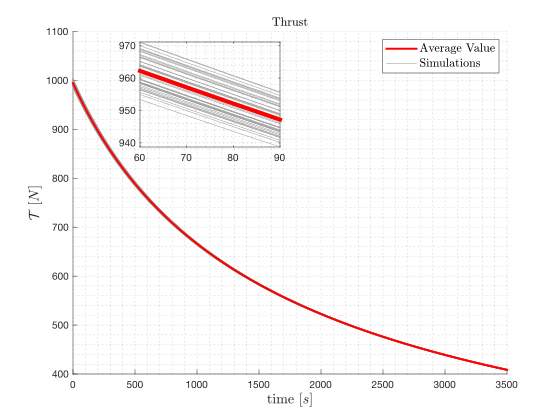
\includegraphics[scale=1]{i/immagini_unc/thrust_unc.svg}
    \caption{default}
    \label{fig:thrust_unc}
    \end{minipage}
    
    \hspace{0.3cm}
    
    
    \begin{minipage}[b]{0.4\linewidth}
    \centering
    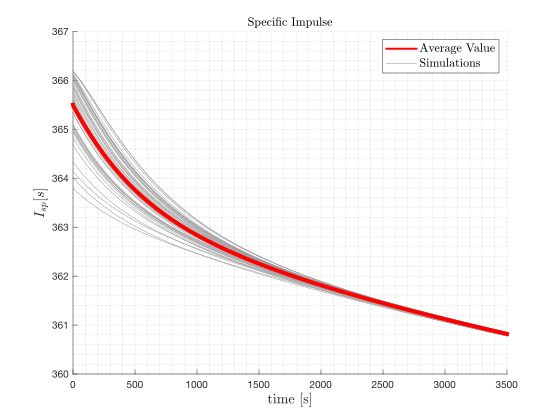
\includegraphics[width=\textwidth]{i/immagini_unc/Isp_unc.svg}
    \caption{default}
    \label{fig:Isp_unc}
    \end{minipage}
    
    \hspace{0.3cm}
    
    \begin{minipage}[b]{0.4\linewidth}
    \centering
    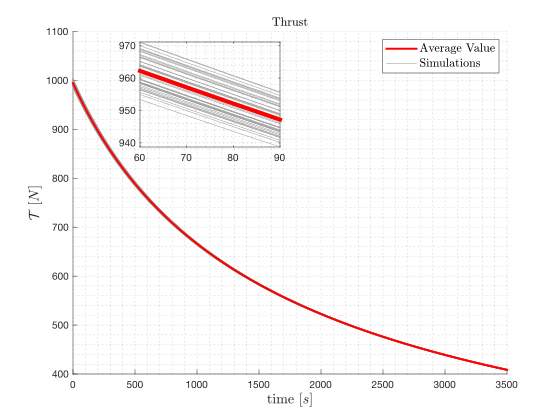
\includegraphics[width=\textwidth]{i/immagini_unc/thrust_unc}
    \caption{default}
    \label{fig:fiof_unc}
    \end{minipage}
    \end{figure}








